\documentclass{article}
\usepackage[utf8]{inputenc}

\title{new}
\author{vranen }
\date{March 2020}

\usepackage{natbib}
\usepackage{graphicx}

\begin{document}

\maketitle

\section{Introduction}
There is a theory which states that if ever anyone discovers exactly what the Universe is for and why it is here, it will instantly disappear and be replaced by something even more bizarre and inexplicable.
There is another theory which states that this has already happened.

\section{Notes}
Overview
The FSM (Finite State Machine) is available as a mixin for the Akka Actor and is best described in the Erlang design principles

A FSM can be described as a set of relations of the form:

State(S) x Event(E) -> Actions (A), State(S’)

These relations are interpreted as meaning:

If we are in state S and the event E occurs, we should perform the actions A and make a transition to the state S’.

\begin{figure}[h!]
\centering
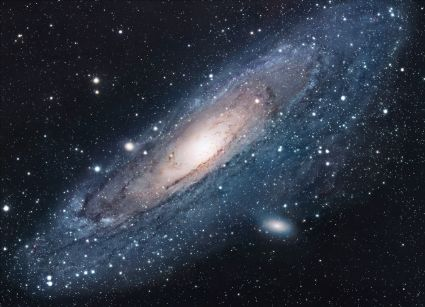
\includegraphics[scale=1.7]{universe}
\caption{The Universe}
\label{fig:universe}
\end{figure}

\section{Conclusion}
``I always thought something was fundamentally wrong with the universe'' \citep{adams1995hitchhiker}

\bibliographystyle{plain}
\bibliography{references}
\end{document}
